En 2025, dans une ville, le club de basketball comptait 900 adhérents. On estime que chaque année, le club perd 10 adhérents.
	
	On note $B_{n}$ le nombre d'adhérents au club de basket l'année $2025+n$.
	
	\begin{enumerate}
		\item Calculer $B_{1}$ et interpréter le résultat.
		\item Exprimer $B_{n}$ en fonction de $n$.
		\item Justifier que le club aura perdu plus de $10~\%$ de ses adhérents entre 2025 et 2035.
	\end{enumerate}
	
	Dans cette même ville en 2025, le club de handball comptait 200 adhérents.
	
	Pour les années suivantes, on estime que le nombre d'adhérents au club de handball peut être représenté par le graphique suivant :
	
	\begin{center}
		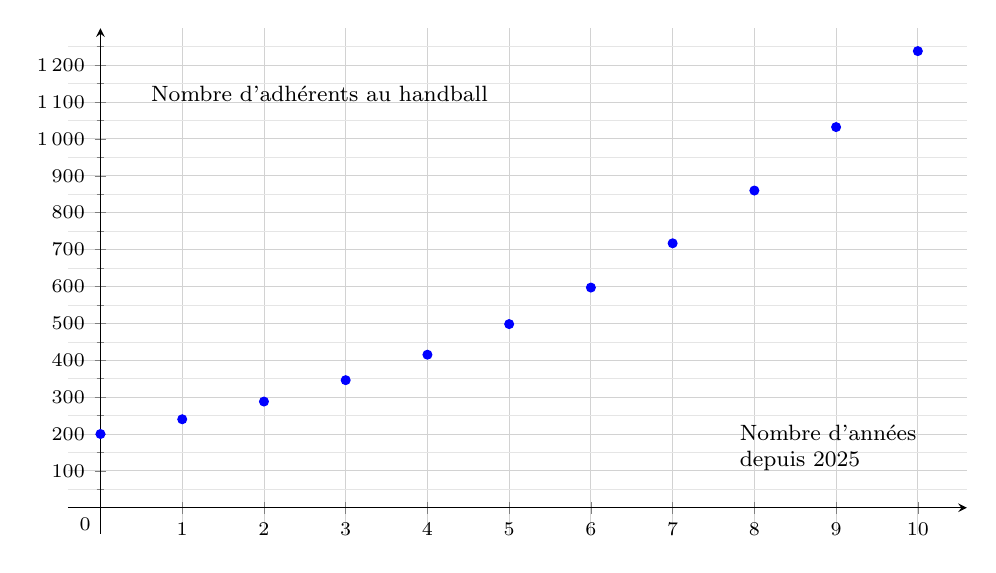
\begin{tikzpicture}
		
		
			\begin{axis}[/pgf/number format/.cd, use comma,1000 sep={\,},
				width=13cm,height=8cm,
				xmin=-0.4,xmax=10.6,ymin=-70,ymax=1300,
				xtick={0,1,2,3,4,5,6,7,8,9,10},
				ytick={0,100,200,300,400,500,600,700,800,900,1000,1100,1200},
				minor ytick={50,150,250,350,450,550,650,750,850,950,1050,1150,1250},
				tick label style={font=\scriptsize},
				grid=both, axis lines=center,
				grid style={gray!35,line width=0.3pt},
				minor grid style={gray!20,line width=0.2pt}]
				\addplot[only marks,mark=*,mark size=1.6pt,color=blue] coordinates {
					(0,200) (1,240) (2,288) (3,346) (4,415) (5,498)
					(6,597) (7,717) (8,860) (9,1032) (10,1238)};
				\node[above right] at (axis cs:0.5,1075) {\footnotesize Nombre d'adhérents au handball};
				\node[below right] at (axis cs:7.5,260) {\footnotesize\begin{tabular}{l}Nombre d'années\\depuis 2025\end{tabular}};
				\node[below left] at (axis cs:0,0) {\scriptsize 0};
			\end{axis}
		\end{tikzpicture}
	\end{center}
	
	\begin{enumerate}[start=4]
		\item Par lecture graphique, estimer, avec la précision permise par le graphique, le nombre d'adhérents au club de handball en 2028.
		\item On modélise le nombre d'adhérents au club de handball l'année $2025+n$ par $H_{n}$ et on admet que, pour tout entier naturel $n$, $H_{n+1}=1{,}2\times H_{n}$. Quelle est la nature de la suite $\left(H_{n}\right)$ ? Préciser son premier terme et sa raison.
		\item À partir de quelle année le nombre d'adhérents au club de handball sera supérieur au nombre d'adhérents au club de basketball ? Justifier la réponse.
	\end{enumerate}
